\documentclass[letterpaper,10pt]{article}
\usepackage{graphicx}
\usepackage[export]{adjustbox}
\usepackage{fancyhdr}
\usepackage[spanish]{babel}
\usepackage{listings}
\usepackage[utf8]{inputenc}
\pagenumbering{roman}
\usepackage[left=2.5cm,
top=2.5cm,
right=2.5cm,
bottom=3cm]{geometry}
\usepackage{listings}
%\pagenumbering{gobble}
\usepackage{ragged2e} 
%\usepackage{fancy}
\usepackage{placeins}
\pagestyle{fancy}
\fancyhf{}
\usepackage[spanish]{babel}
\usepackage[utf8]{inputenc}
\usepackage[left=2.5cm,
top=2.5cm,
right=2.5cm,
bottom=3cm]{geometry}

%Portada
\begin{document}
	
\begin{titlepage}
	
	\begin{center}
		\vspace*{-1in}
		\begin{figure}[htb]
			\centering
			
\includegraphics[scale=1.5]{ESCUDO}
		\end{figure}
		
		\textbf{TECNOLÓGICO NACIONAL DE MÉXICO}\\
		\vspace*{0.15in}
		INSTITUTO TECNOLÓGICO DE MORELIA \\
		\vspace*{0.3in}
		\begin{large}
			DEPARTAMENTO DE INGENIERÍA ELECTRÓNICA\\
		\end{large}
		\vspace*{0.2in}
		\begin{large}
			CONTROL I\\
		\end{large}
		\vspace*{0.3in}
		\begin{Large}
			\textbf{PRACTICA DE LABORATORIO No.2: \\
			Polos y Ceros encontrados por Inspección}\\ 
		\end{Large}
		\vspace*{0.3in}
		\begin{large}
		\textbf{PROFESOR:} GERARDO MARX CHÁVEZ CAMPOS\\
		\end{large}
		\vspace*{0.2in}
		\begin{large}
			JESÚS ANTONIO MAGAÑA SILVA: \textbf{14121126}\\
			VÍCTOR HUGO GARCÍA VALDIVIA: \textbf{14121088}
		\end{large}
		\vspace*{0.3in}
		\rule{80mm}{0.1mm}\\
		\vspace*{0.1in}
		\begin{large}
			MORELIA, MICHOACÁN \\
			NOVIEMBRE, 2017 \\
		\end{large}
	\end{center}
\end{titlepage}

	%Introduccion
	\pagebreak
	\justify
	\pagebreak
	\pagenumbering{arabic}
	\section{Introducción}
	\vspace*{0.3in}
	El objetivo de la práctica es poder apreciar, conocer y manipular los distintos métodos para encontrar o identificar los polos y ceros a traves de la función de transferencia o por el método de inspección, se tienen dos circuitos (1) y (2) los cuales seran analizados por estos metodos para encontrar sus polos y ceros.
	
	%Figura\ref{fig: Foto 2}
	\begin{figure}[h!]
		\centering
		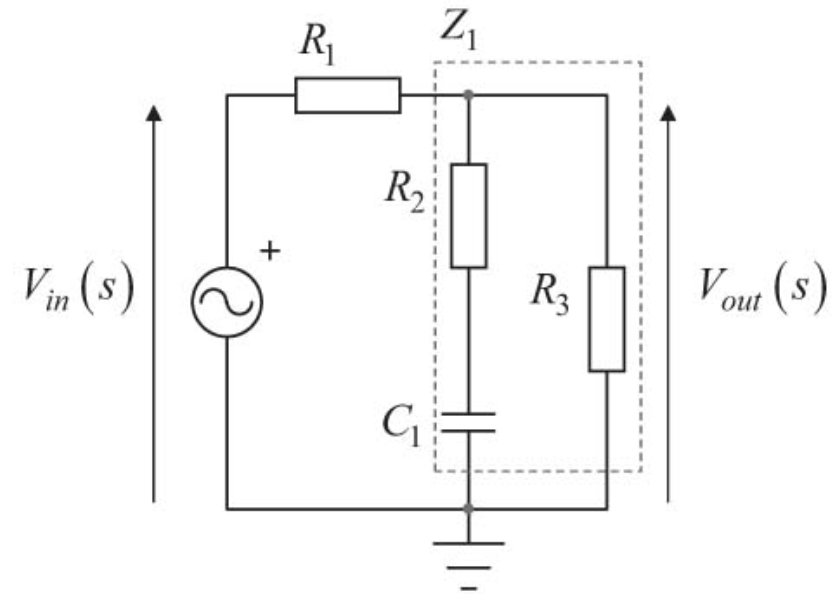
\includegraphics[scale=0.4]{CIRCUITORC}
		\caption{Esquema deL circuito RC}
	%	\label{fig: Foto 2}
	\end{figure}
	
		\vspace*{0.3in}
	
	Mostrando las diferencias entre las formas de onda entre la respuesta de un circuito respecto al otro.
	
	%Figura\ref{fig: Foto 2}
	\begin{figure}[h!]
		\centering
		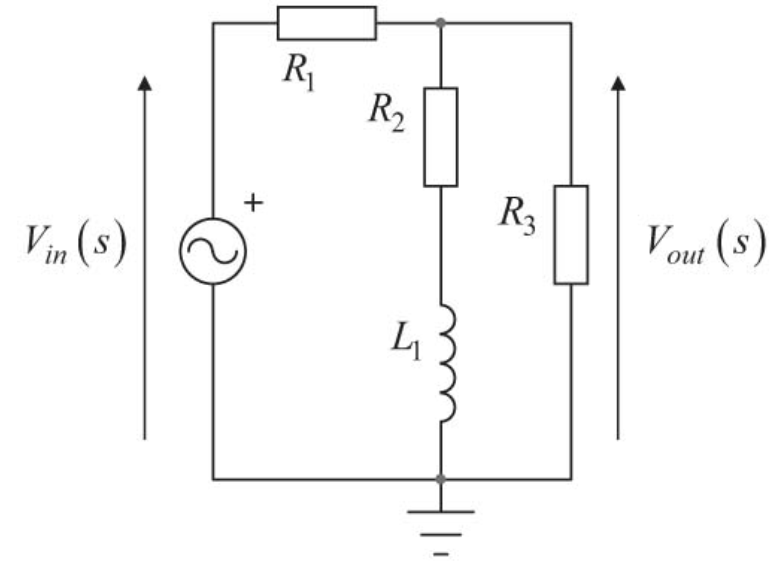
\includegraphics[scale=0.4]{CIRCUITORL}
		\caption{Esquema del circuito RL}
		%	\label{fig: Foto 2}
	\end{figure}



	
	%Metodologia
	\pagebreak
    \section{Metodología}
    %\begin{itemize}
    \vspace*{0.3in}	
    %\end{itemize}
    
    Se realizará primero el análisis del circuito RC
    \vspace*{0.3in}
    
    \begin{itemize}
    	\item
    	\textbf{CIRCUITO RC}\vspace*{0.4in}\\
    	Observe que una fuente de CA Vin está entregando una señal a través de una resistencia R1 a una red hecha de una combinación serie-paralelo de dos resistencias y un condensador.
    	Hay un elemento de almacenamiento distinto C1; esta es una red de primer orden.
    	Sin embargo, es difícil saber dónde hay polos o ceros, sin embargo, debe
    	adaptarse al formato dado por:
    \end{itemize}
    %	Figura\ref{fig: Foto 1}
    \vspace*{0.2in}
    	\begin{figure}[h!]
    		\centering
    		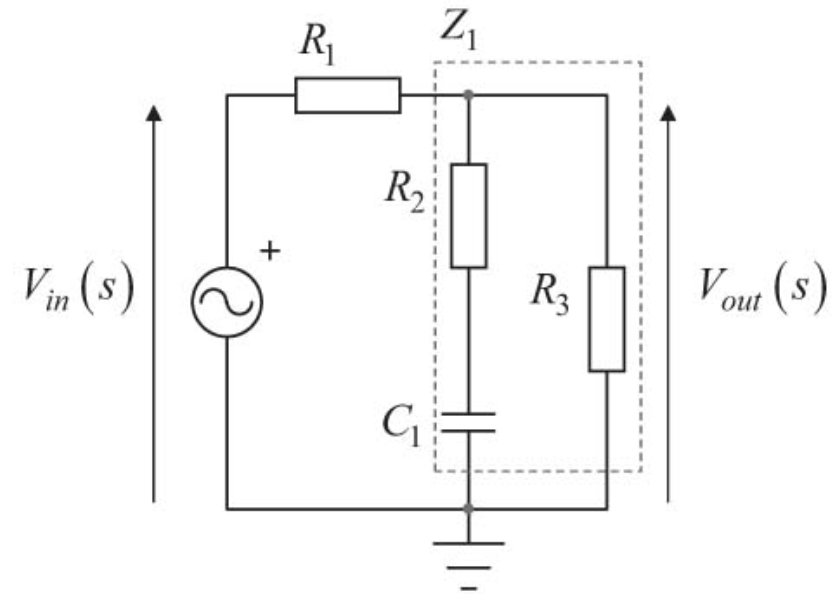
\includegraphics[scale=0.4]{CIRCUITORC}
    		\caption{Diagrama del Circuito RC}
    %		\label{fig: Foto 1}
    	\end{figure}

        \vspace*{0.3in}
    \begin{equation}
    H(s) = \frac {V_{out}}{V_{in}} \rightarrow Go \frac {(1+ \frac{S}{W_{Z1}})}{(1+ \frac{S}{W_{P1}})}\\  
    \end{equation}
    
     \begin{itemize}
    	\item
    	\textbf{BIAS POINT (DC)}\vspace*{0.4in}\\
		Es posible obtener por "fuerza bruta" la expresión de impedancia Z1 y
		aplicando la expresión del divisor de voltaje:
		
   		\begin{equation}
		V_{out} = V_{in}(s) \frac {R_3}{R_1 + R_3}\rightarrow \frac {V_out}{V_in}= Go= \frac {R_3}{R_1 + R_3}\\  
		\end{equation}
     \end{itemize}

	\pagebreak
	A continuación se muestra (4) el circuito analizado en CD del circuito RC:
	\vspace*{0.3in}
    \begin{figure}[h!]
    	\centering
    	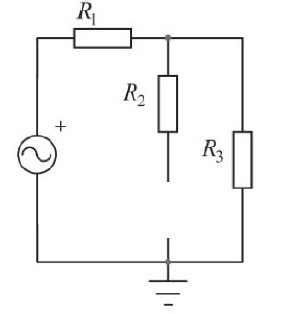
\includegraphics[scale=0.7]{CIRCUITORCDC}
    	\caption{Diagrama del Circuito RC EN CD}
    	%		\label{fig: Foto 1}
    \end{figure}

     
    \begin{itemize}
    	\item
    	\textbf{CEROS}\vspace*{0.4in}\\
    	Recordando la definición de cero, es un punto de frecuencia en el que
    	la excitación ya no alcanza la salida.
    	
    	O bien un elemento en serie con la señal ofrece una impedancia infinita a un cierto
    	frecuencia o un elemento que une la ruta de señal al suelo se convierte en un corto
    	circuito, de nuevo en un cierto punto de frecuencia. En nuestro ejemplo, el único elemento que
    	puede detener la señal de llegar a la salida es la combinación en serie de $R_2$ y $C_1$.\\ 
    	Cuando su impedancia resultante es nula (cortocircuito), tenemos un cero en el
    	función de transferencia:
    	
    	\begin{equation}
    	R_2+ \frac{1}{sC1}=0 \\  
    	\end{equation}
    
        \begin{equation}
   	 	\frac{R_2C_1+1}{sC1}=0 \\  
    	\end{equation}
    	
    	\begin{equation}
    	R_2C_1+1=0 \\  
    	\end{equation}
   
    	Teniendo el valor de $W_Z1$.
    	\begin{equation}
		W_{Z1}=\frac{1}{R_2C1} \\  
		\end{equation}
		
		Con esto se puede tener la siguiente ecuación:
		\begin{equation}
		Go= \frac {N(s)}{D(s)}\rightarrow \frac {R_3}{R_1 + R_3}*\frac {(1 + sR_2C_1)}{D(s)}\\  
		\end{equation}
		
		Teniendo el valor de $W_{P1}$:
		\begin{equation}
		W_{P1}=\frac {1}{Tau}=\frac {1}{R_{eq1}C_1}\\  
		\end{equation}
		
		\begin{equation}
		W_{P1}=\frac {1}{(R_2+R_1//R_3)C_1}\\  
		\end{equation}
		
		Quedando de la siguiente manera
		\begin{equation}
		Go=\frac {R_3}{R_1 + R_3}*\frac {(1 + sR_2C_1)}{(R_2+R_1//R_3)(Cs+1)}\\  
		\end{equation}
		
		\end{itemize}

    \begin{equation}    
    G(S) = \frac{W_i(S)}{H(S)}
    \end{equation}
    \begin{equation}
    G(S) = H(S)(\frac{1}{\frac{1}{R} + CS})
    \end{equation}
	\begin{equation}
	W_i(S) = H(S)(\frac{1}{R} + CS)
	\end{equation}
	 \begin{equation}
	G(S) = H(S)(\frac{1}{C\frac{1}{RC} + CS}) = \frac{\frac{1}{c}}{s+\frac{1}{RC}}
	\end{equation}
    
    En la práctica se obtuvo la siguiente curva característica de carga del capacitor, en la cual se observa en la siguiente imagen, resaltando el Tao que se midió por cursores calculando el 65 porciento del voltaje máximo de carga y el comienzo de carga.
    %	Figura\ref{fig: Foto 1}
    \vspace*{0.2in}
    \begin{figure}[h!]
    	\centering
    	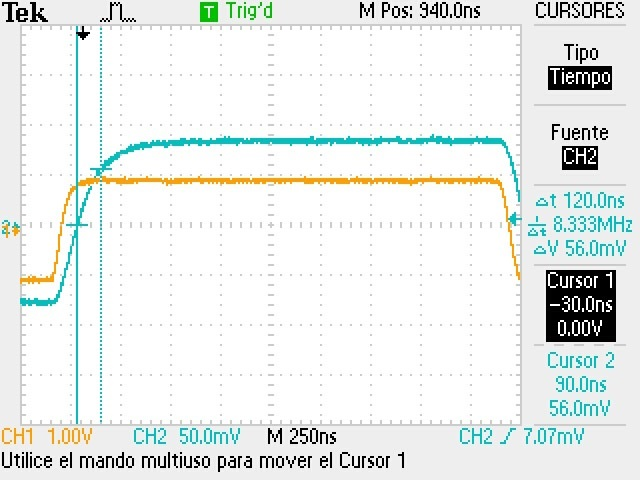
\includegraphics[scale=1.5]{TAOCAP}
    	\caption{Diagrama de la gráfica obtenida con las mediciones en respuesta del tiempo de carga del capacitor(Circuito RC).}
    	%		\label{fig: Foto 1}
    \end{figure}
    \begin{itemize}
    	\item
    	\textbf{CIRCUITO RL}\vspace*{0.4in}\\
    	En este circuito simplemente cambiamos del circuito anterior el capacitor por un inductor, este inductor lo modificamos por uno de $6.58 mH$.
    	Para analizarlo primero fué por inspección.
    	\end{itemize}
    
     %	Figura\ref{fig: Foto 1}
    \vspace*{0.2in}
    \begin{figure}[h!]
    	\centering
    	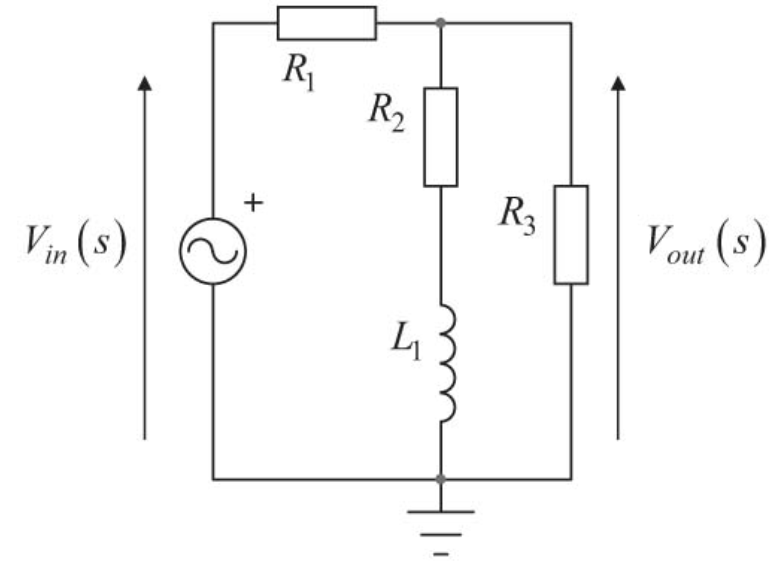
\includegraphics[scale=0.4]{CIRCUITORL}
    	\caption{Diagrama del Circuito RL}
    	%		\label{fig: Foto 1}
    \end{figure}
    
     \begin{equation}
       Vout(S) = \frac{Vin(S)R1||R2}{R1+R2||R3}
    \end{equation}
     \begin{equation}
    \frac{Vout(S)}{Vin(S)} = \frac{R2||R3}{R1+R2||R3}
    \end{equation}
   
    
    
    Para $W = z1$
    

	\begin{equation}
		R2 + SL = 0
	\end{equation}
    
    \begin{equation}
    R2 ( 1 + \frac{SL}{R2}) = 0
    \end{equation}
    
     \begin{equation}
    1 + (\frac{SL}{R2})=0
    \end{equation}
    
     \begin{equation}
    Wz1 = \frac{R2}{L}
    \end{equation}
    
     \begin{equation}
    Wp1 = \frac{R2+R1||R3}{L}
    \end{equation}
    
     \begin{equation}
    H(S)= \frac{R2||R3}{R1+R2||R3}\frac{1+S\frac{L}{R2}}{1+S\frac{L}{R2+R1||R3}}
    \end{equation}
    
      
     	Ahora se analizará de manera algebraica y teóricamente se debe llegar a lo mismo que el análisis de inspección llegando a lo mismo que la ecuación 22.
	    Haciendo una resistencia en serie equivalente de R2 con la bobina se tiene que:
      
    \begin{equation}
    Req1 = R2 + SL
    \end{equation}
    
    \begin{equation}
    Rp1 = \frac{R3(R2 + SL)}{R3 + R2 + SL}
    \end{equation}
    
    \begin{equation}
    Vout (S) = \frac{Vin(\frac{R3(R2+SL)}{R3+R2+SL})}{R1\frac{R3(R2+SL)}{R3+R2+SL}} 
    \end{equation}

	\begin{equation}
	\frac{Vout}{Vin} = \frac{R3(R2+SL)}{R1R3+R1R2+R1SL+R3R2+R3SL}
	\end{equation}
	
	\begin{equation}
	\frac{Vout}{Vin} = \frac{R3R2(1+\frac{SL}{R2})}{R1(R3+R2)+R3R2+R1SL+R3SL}
	\end{equation}
	
	\begin{equation}
	\frac{Vout}{Vin} = \frac{R3R2(1+\frac{SL}{R2})}{(R1(R3+R2)+R3R2)(1+\frac{R1SL+R3SL}{(R1(R3+R2)+R3R2)})}
	\end{equation}	
	
	\begin{equation}
	\frac{Vout}{Vin} = \frac{R3R2(1+\frac{SL}{R2})}{(R1(R3+R2)+R3R2)(1+\frac{SL(R1+R3)}{(R1R3+R1R2+R3R2)})}
	\end{equation}
	
	\begin{equation}
	Wz1=R2
	\end{equation}
	
	\begin{equation}
	Wp1 = \frac{(R1R3+R1R2+R3R2)}{L(R1+R3)}
	\end{equation}
	
	\vspace*{0.4in}	
	    Con los datos recabados en la práctica y medidos con el osciloscopio se muestran en la siguiente tabla y a continuación la gráfica obtenida y generada del circuito RL.\\
   

    \begin{center}
    	\begin{tabular}{|c|c|c|}
    		\hline 
    		Frecuencia & $V_{in}$ & $V_{out}$  \\ 
    		\hline 
    		$1 Hz$  & 0.464 & 0.391 \\
    		\hline 
    		$2 Hz$  & 0.464 & 0.391 \\
    		\hline 
    		$3 Hz$  & 0.464 & 0.391 \\
    		\hline 
    		$4 Hz$  & 0.464 & 0.391 \\
    		\hline 
    		$5 Hz$  & 0.464 & 0.391 \\
    		\hline 
    		$6 Hz$  & 0.464 & 0.391 \\
    		\hline 
    		$7 Hz$  & 0.464 & 0.391 \\
    		\hline 
    		$8 Hz$  & 0.464 & 0.391 \\
    		\hline 
    		$9 Hz$  & 0.464 & 0.391 \\
    		\hline 
    		$10 Hz$  & 0.464 & 0.391 \\
    		\hline 
    		$20 Hz$  & 0.464 & 0.391 \\
    		\hline 
    		$30 Hz$  & 0.464 & 0.392 \\
    		\hline 
    		$40 Hz$  & 0.464 & 0.392 \\
    		\hline 
    		$50 Hz$  & 0.464 & 0.392 \\
    		\hline 
    		$60 Hz$  & 0.464 & 0.392 \\
    		\hline 
    		$70 Hz$  & 0.464 & 0.392 \\
    		\hline 
    		$80 Hz$  & 0.464 & 0.392 \\
    		\hline 
    		$90 Hz$  & 0.464 & 0.392 \\
    		\hline 
    		$100 Hz$  & 0.464 & 0.392 \\ 
    		\hline 
    		$200 Hz$  & 0.464 & 0.393 \\
    		\hline 
    		$300 Hz$  & 0.464 & 0.393 \\
    		\hline
    		$400 Hz$  & 0.464 & 0.393 \\
    		\hline 
    		$500 Hz$  & 0.464 & 0.393 \\
    		\hline 
    		$600 Hz$  & 0.464 & 0.393 \\
    		\hline 
    		$700 Hz$  & 0.464 & 0.393 \\
    		\hline 
    		$800 Hz$  & 0.464 & 0.3935 \\
    		\hline 
    		$900 Hz$  & 0.464 & 0.3935 \\
    		\hline 
    		$1 kHz$  & 0.464 & 0.3935 \\
    		\hline 
    		$2 kHz$  & 0.464 & 0.395 \\
    		\hline 
    		$3 kHz$  & 0.464 & 0.396 \\
    		\hline 
    		$4 kHz$  & 0.464 & 0.397 \\
    		\hline 
    		$5 kHz$  & 0.464 & 0.397 \\
    		\hline 
    		$6 kHz$  & 0.464 & 0.398 \\
    		\hline
    		$7 kHz$  & 0.464 & 0.398 \\
    		\hline 
    		$8 kHz$  & 0.464 & 0.4 \\
    		\hline 
    		$9 kHz$  & 0.464 & 0.403 \\
    		\hline 
    		$10 kHz$  & 0.464 & 0.405 \\
    		\hline 
    		$20 kHz$  & 0.464 & 0.416 \\
    		\hline 
    		$30 kHz$  & 0.464 & 0.424 \\
    		\hline 
    		$40 kHz$  & 0.464 & 0.428 \\
    		\hline 
    		$50 kHz$  & 0.464 & 0.43 \\
    		\hline 
    		$60 kHz$  & 0.464 & 0.431 \\
    		\hline 
    		$70 kHz$  & 0.464 & 0.4314 \\
    		\hline 
    		$80 kHz$   & 0.464 & 0.432 \\
    		\hline 
    		$90 kHz$   & 0.464 & 0.4325 \\
    		\hline 
    		$100 kHz$  & 0.464 & 0.4325 \\
    		\hline 
    		$200 kHz$  & 0.464 & 0.4325 \\
    		\hline 
    		$300 kHz$  & 0.464 & 0.4325 \\ 
    		\hline 
    		$400 kHz$  & 0.464 & 0.432 \\
    		\hline 
    		$500 kHz$  & 0.464 & 0.428 \\
    		\hline 
    		$600 kHz$  & 0.464 & 0.425 \\
    		\hline 
    		$700 kHz$  & 0.464 & 0.420 \\
    		\hline 
    		$800 kHz$  & 0.464 & 0.415 \\
    		\hline 
    		$900 kHz$  & 0.464 & 0.410 \\
    		\hline 
    		$1 MHz$  & 0.464 & 0.408 \\
    		\hline
    	\end{tabular} 
    \end{center}

 

 %	Figura\ref{fig: Foto 1}
\vspace*{0.2in}
\begin{figure}[h!]
	\centering
	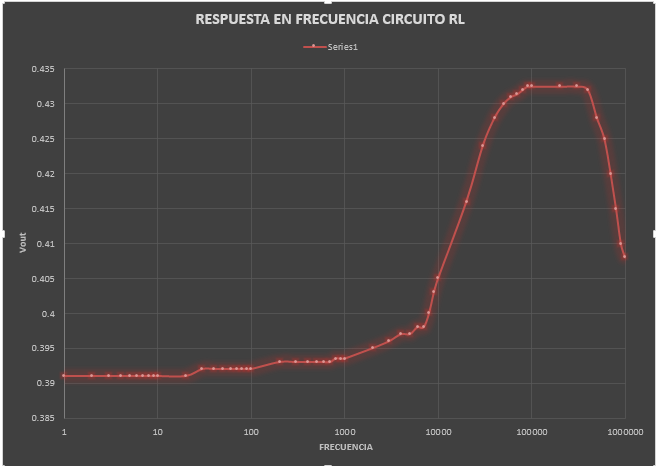
\includegraphics[scale=0.9]{RESPUESTAEN}
	\caption{Diagrama de la gráfica obtenida con las mediciones en respuesta de la frecuencia(Circuito RL).}
	%		\label{fig: Foto 1}
\end{figure}

 \pagebreak
 
 
 %Codigo
 \section{Código}
\begin{center}
	En este apartado se usó PSpice A/D Metiendo los valores correspondientes entre cada nodo
	\begin{lstlisting}[frame=single]
	
	;First Circuit LC:
	V1  1  0  ac 1
	R1	1  2  1000
	R2  2  3  1000
	L1  3  0  6.58mH
	R3  2  0  1000
	.ac DEC 100  100  1000K
	.probe
	.end
	
	\end{lstlisting}
	
	 %	Figura\ref{fig: Foto 1}
	\vspace*{0.2in}
	\begin{figure}[h!]
		\centering
		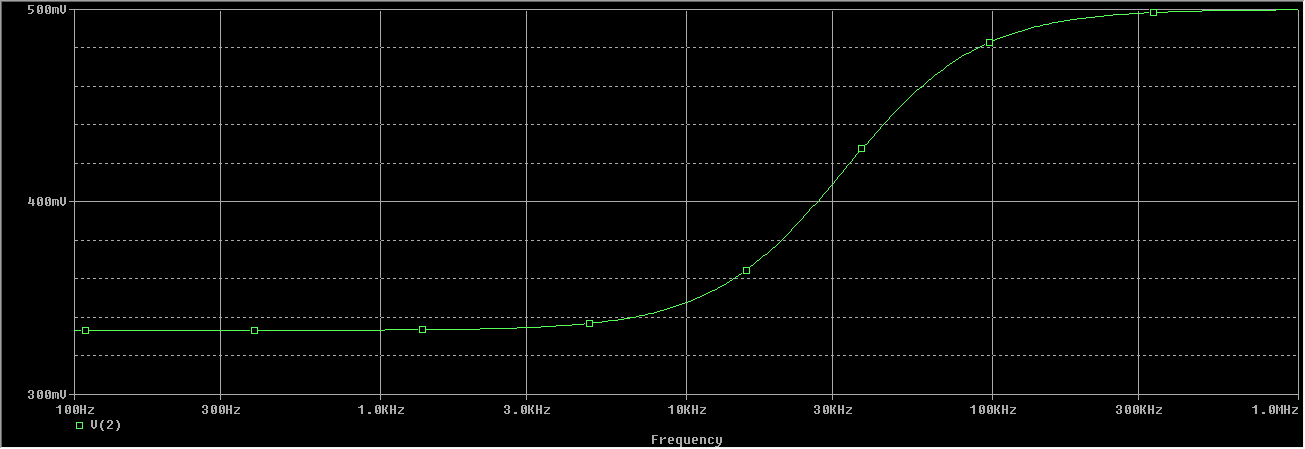
\includegraphics[scale= 0.45]{ORCADRLSIMULATE}
		\caption{Gráfica generada por OrCAD Spice}
		%		\label{fig: Foto 1}
	\end{figure}
	
\end{center}
\FloatBarrier


\vspace*{0.3in}
\textbf{}
Gracias al código anterior se pueden mostrar las gráficas siguientes donde se muestra la curva en dB en el circuito RL\\

%\vspace*{0.5in}
%\begin{itemize}[here!]
%\item Wi = Wo
%\end{itemize}



%Conclusion
\newpage

\section{Conclusiones}
\vspace*{0.3in}
\textbf{Victor Hugo Garcia valdivia\\}
En esta práctica se puede concluir que un circuito de segundo orden se puede resolver con un análisis de inspección o por análisis algebraico. Y efectivamente da lo mismo, sólo en la práctica (implementado el circuito) no es tan precisa la gráfica que deberíamos de haber obtenido pero sí algo parecido, esto debido a que los valores del inductor, el mismo generador, el ruido, etc. Nos generan discrepancia entre lo calculado-simulado con lo real. \\

	 
\vspace*{0.3in}
	  
\textbf{Jesús Antonio Magaña Silva} \\

Durante la realización de esta práctica fue posible detectar tanto por 
el método de inspección asi como el método algebraico los polos y ceros
nuestro sistema que en este caso fueron unos circuitos RL y RC viendo
las diferencias entre uno y otro.
Coincidiendo la simulación con lo práctico formando una gráfica con los 
diversos valores de frecuencias y voltajes de salida nos pudimos dar 
cuenta que al final queda de la misma manera quedando mas definida la 
grafica en la simulación, ademas como lo  pudimos ver en clase el metodo 
algebraico fue mas dificil que por el método de inspección.
Otro aspecto que se notó que a grandes frecuencias en el rango de los
Megas la respuesta del inductor es cuando se tiene la decaida despues de 
tener el valor maximo constante mostrando una grafica rn forma muy parecida
a una campana.\\
\end{document}